\documentclass[12pt]{article}
\usepackage[parfill]{parskip}
\usepackage{graphicx} %for inserting images
\usepackage{float}
\usepackage{caption}
\usepackage{subcaption}
\usepackage{setspace}
\usepackage[a4paper, total={5.75in, 8in}]{geometry}
\graphicspath{{../plots/}}
\bibliographystyle{apalike}
\onehalfspacing

\date{}

\begin{document}

\begin{titlepage}

  \begin{minipage}[t]{0.5\textwidth}
    \raggedright
    \large
    Sam Smith
  \end{minipage}%
  \begin{minipage}[t]{0.5\textwidth}
    \raggedleft
    \large
    August 2024
  \end{minipage}

  \vspace{0.6in}
  
  \begin{center}
    
\includegraphics[width=0.5\textwidth]{imperiallogo.jpg}
  \end{center}
  
  \vspace{0.5in}
  
  \rule{\linewidth}{1.2mm}
  \begin{center}
    \LARGE
    \textbf{Phylogenetic Backbone Reconstruction using Kmeans Clustering on Coleopteran Mitogenomes}
  \end{center}
  \rule{\linewidth}{1.2mm}
  
  \vspace{0.5in}
  
  \begin{center}
    \large Supervisor: Alfried Vogler \\ Department of Life Sciences \\ Imperial College London \\ SW7 2AZ \\ UK
  \end{center}
  
  \vspace{0.6in}
  
  \begin{center}
    \large A thesis submitted in partial fulfilment of the requirements for the degree of Master of Science at Imperial College London - submitted for the MSc in Computational Methods in Ecology
  \end{center}

\end{titlepage}

\onehalfspacing
\setcounter{tocdepth}{2}

\newpage
\textbf{\large Declaration:}

The data used in this study was provided by the Site 100 database, hosted by the Natural History Museum, London, in collaboration with Imperial College London. The data required a minimal extent of cleaning; merely just correcting typo errors and changing file type (i.e. GenBank to Fasta). The SigClust algorithm developed and scrutinized further in this study was originally published by Chappell et al., 2017. All analysis, data cleaning, plotting, and thesis writing was entirely independant, unless otherwise explicitly stated in the text. 

\newpage
\tableofcontents

  \newpage
  \section{Abstract}
  The challenge of building large phylogenetic trees is not new, but increasingly frustating due to the growing availability of molecular data. This investigation explores the application of kmeans clustering in aiding the reconstruction of large phylogenies. In particular, Coleopteran mitogenomes from The Site 100 database served as the sequences used to develop the method in this investigation. The method proposed in this study aims to cluster sequences and compute the `cluster centers' that can consequently serve as representatives for phylogenetic backbone reconstruction. Therefore, the phylogenies of individual clusters (subtrees) can be added to their respective tip on the backbone, thus providing additional phylogenetic detail where desired. Two clustering approaches were experimented in this study: a simple kmeans approach and an adapted version of a previously developed algorithm that also takes advantage of the speed and simplicity of kmeans clustering. The simple approach whereby kmeans was executed directly on a distance matrix struggled to find suitable representatives for bacbone reconstruction. However the implementation of signal clustering method (SigClust) showed more promise. Whilst the clusters from this method  were mostly not taxonomically homogenous and therefore unlikely to be monophyletic and serve as good subtrees, the cluster representatives did manage to capture a lot of the diversity present in the sample. Despite the disapointing contents of each cluster, there were cases of good taxonomically pure clusters which were used to illustrate the addition of subtrees onto a phylogenetic backbone. 
  
  \newpage
  \section{Introduction}
    
  Coleoptera consists of a quarter of all known animal species on Earth \cite{YUAN201699}. There are around 400,000 described beetle species in this highly diverse order. The order has been subject to many phylogenetic analyses based on morphology and more recently through the 21st Century, molecular data \cite{orlov}. Understanding phylogeny has broad implications in ecology, particularly relating to ecosystem services, pathogen-host interactions, and general community structure \cite{Davis2010}. Moreover, applying a phylogenetic framework to phenological studies provides insight into the behaviour of closely related organisms, particularly important for understanding their response to climate change \cite{Davis2010}. Coleopterans are found in all climates and habitats except the most extreme latitudes and altitudes \cite{brit}; they strongly contribute to ecosystem services in almost all terrestrial and freshwater ecosystems \cite{Zhang2018}. Investigating the complex phylogeny of Coleopterans is fundamental to understanding the processes that has led to this extraordinary diversity \cite{Zhang2018}.
  
  Determining Coleopteran phylogeny has been challenging due the sparse availability of molecular data relative to the species richness of the order \cite{Zhang2018}. Whilst studies continue to refine the phylogenetic tree and clarify evolutionary relationships between species; previous phylogenetic reconstructions of the order have provided the monophyly of the four described suborders: Archostemata, Adephaga, Myxophaga, and Polyphaga. The extreme species richness of Coleoptera, coupled with the computational limitations of traditional tree building software, suggests the need for innovative phylogenetic methods to be developed. For example, the computational burden placed on phylogentic software increasingly worsens upon the addition of species \cite{ahmed}. This is particularly frustrating in an era of increasingly available molecular data \cite{Sanderson2003}. However, the challenge of building large trees is not new and methods have been developed to address these challenges. For example, less dense sampling leading to the development of strongly supported phylogenetic backbones, that capture the broad diversity of a clade without including the detail of every species has become popular practice. It provides means for a consistent classification for further research \cite{Xu2022}. However, these backbone trees not only fail to capture all of the evolutionary detail, they also do not facilitate the addition of such. The novel method proposed in this study is a `divide-and-conquer' approach, aimed to divide the available phylogentic detail at the tip of a tree through clustering, and graft onto a backbone phylogeny where appropriate.
  
  Clustering algorithms are frequently employed to classify genetic data into groups based on similarity. These clusters can then be analysed individually, or a meta-analysis can be conducted using representative sequences from each cluster. This method reduces computational demands, making it a more efficient solution to observe broader evolutionary relationships than analyzing an entire dataset. One popular clustering tool that has not found a mainstream application in phylogenetic reconstruction is kmeans. Kmeans is a fast, effective and straightforward algorithm well-employed in other areas of biological research \cite{lu04}; it partitions data through an iterative process into a predefined number of clusters based on shared variables. One of the few examples of kmeans being used in phylogenetic research is by Chappell et al., (2017). The aim of this study was to cluster sequences from highly diverse environmental samples quickly and alignment free, for consequent analyses to take place. This study converted DNA sequences into kmers and then transformed them into an intermediate binary format before kmeans clustering \cite{Chappell2017}. This innovative approach clustered sequences with high accuracy, thus making a strong case for kmeans clustering to be used more in this field. Whilst the absence of an alignment in this method makes it incredibly fast, this method has its drawbacks. Firstly, reducing the detail in the sequences during the conversion to a binary vector format, suggests the algorithm is unsuited for a closely related sample of sequences. Secondly, the application of the SigClust software is currently unsuitable for bacbone reconstruction as it does not provide a means for selecting representatives from each cluster.

  This is an exploratory investigation that describes a novel method for building large phylogenetic trees whilst also building on the work of Chappell et al (2017). The study particularly provides a solution to the challenge of building very large trees by efficiently combining multiple phylogenetic trees that are originally designed to be grafted together - unlike previous methods. As the need for constructing larger phylogenetic trees grows, it is certain that to include more species, increasing the number of sites per species is essential - but not always possible. To combat this,  `supertree' methods such as matrix representation with parsimony (MRP) \cite{MRP}, or MinCut \cite{MinCut} have been used to combine `input' trees that contain overlapping taxanomic coverage. The method to build large trees proposed in this study is a logical step-by-step process that combines using kmeans clustering for backbone tree reconstruction with consequent tree grafting. The method suggests smaller monophyletic `subtrees' (from samples identified through clustering) that capture less biodiversity will be grafted to the broader backbone tree in their appropriate position. Or equally, one could observe a diverse backbone tree alongside smaller trees that give more detail where desired.
  
  This study aims to find the most appropriate representatives for phylogenetic backbone reconstruction (PBR) utilizing a novel k-means approach as well as an adapted version of the SigClust algorithm. Choosing representatives for backbone reconstruction that include the broader biodiversity within a sample of organisms is a challenge for phylogeneticists. Representatives may be chosen based on morphology, taxonomy, a genetic basis, or a combination \cite{orlov}. Alternatively, representatives do not need to be chosen and backbone trees can be proposed as just a pruned complete phylogenetic tree, consisting of only strongly supported nodes and branches \cite{creedy2024}. Picking representatives based on morphology requires the close inspection of specimens and assumes their capture; in addition, using organisms taxonomy requires the effort of labeling data, potentially even at the cost of an expert taxonomist. Therefore, identifying species for backbone reconstruction using exclusively molecular data is favourable, and takes advantage of the accessibility of new and innovative methods of sequencing specimens. Nuclear or mitogenomes can both used as the molecular data for phylogenetic reconstruction. However, mitochondrial genomes have become increasingly popular for such analyses for reasons including: maternal inheritance and lack of recombination, coupled with a high mutation rate \cite{YU}. Furthermore, this study will be conducted on mitogenomes also due to their greater availability than nuclear genome sequences.
  
  The method developed in this study identifies representatives based solely on their molecular make-up.  This is a more reusable approach, and would eliminate the bias introduced by disparities in species diversity between equivalent taxonomic ranks. The adaptation to the SigClust algorithm, proposed in this study, sacrifices the impressive computational speed for the calculation of cluster centers - which are consequently used as representatives for the backbone phylogenetic tree. The cluster centers will represent the biodiversity of their respective cluster in the backbone phylogenetic reconstruction. Furthermore, upon the construction of a Coleopteran phylogeny using these representatives, additional detail can be added on to the tree by grafting the phylogeny of each separate cluster (subtrees) to its respective backbone tip. This is a flexible and efficient solution to building large trees as subtrees can only be built and added to the backbone wherever is desired and optimal.
  
  It is important to note that despite strong efforts to benchmark the performance of different clustering techniques, it is accepted that the capabilities of different methods are too sensistive to the input data for comparisons between different `clustering' studies to be made \cite{Tseng2007}. Therefore, it is difficult to predict the performance of this study and consequently compare it to others.
  
  \section{Methods}

  All methods in this study were carried out using a combination of R \cite{R} and Python \cite{python}, as well as more specialised software for alignments and phylogenetic analysis. The simplified method is to cluster a set of sequences, choosing the sequence that is most similar to all others in that cluster as the representative for a phylogenetic backbone. Then, subtrees consisting of all the sequences in a particular cluster can be used alongside its respective tip in the backbone to provide additional phylogenetic inference.

    \subsection{Taxon Sampling}

  In this study, Coleopteran mitogenomes were used for developing the method. Sequences were obtained from the Site 100 database, including samples from all around the world \cite{Site100}. Only complete mitogenome sequences labelled `Coleoptera’ were used, resulting in 4438 sequences being extracted from the database, hosted by the Natural History Museum, London. All four suborders were included in the sample, most abundantly represented were Polyphaga and Adephaga - though exact abundances are unknown due to incomplete taxa-specimen labelling in the database. 23 superfamilies were included in the sample with the most represented superfamilies being Chrysomeloidea, Curculionoidea and Staphylinoidea (943,  733, 470 respectively) whilst 413 sequences were not identified to a superfamily level.

    \subsection{Sequence Alignment and Similarity Scoring}

  A sequence alignment is necessary for both the computation of a distance matrix and for consequent tree building. The execution of the SigClust approach does not require an alignment but may benefit from the distance matrix for the identification of cluster centers. For the sequence alignment, all mitogenome sequences were partitioned into their protein coding genes (PCG) before being translated into their respective amino acid sequences. Consequently, a globalpair MAFFT v7.505 \cite{MAFFT} alignment, suitable for closely related sequences of similar lengths was executed. The aligned amino acid sequences were back-translated before clustering and phylogenetic analysis could take place on the aligned nucleotide sequences. Both translation and back-translation were executed using the translate.py and backtranslate.py scripts from the TjCreedy biotools suite \cite{Tjcreedy}. 

  A standard barcode region of the mitochondrial cytochrome C oxidase subunit I gene (COX1) 658bp long \cite{Pent2016} was used for the computation of a distance matrix. This K2P distance matrix would consequently be used for both the simple kmeans and the adapted SigClust approaches. In this study Kimura’s two parameter model (K2P) was used as it is a widely employed model of evolution and a standard for computing distance matrices \cite{Collins}.

  \subsubsection{Kimura's two parameter model}
  The K2P distance between two sequences is calculated as \cite{Kimura1980}:
  \begin{equation}
    K2P = -0.5 \log((1-2P-Q)\sqrt{1-2Q})
  \end{equation}
  where $P$ is the proportion of transitions and $Q$ is the proportion of transversions between two sequences.
  
    \subsection{Clustering and Statistical Analyses}

  Both clustering approaches in this study require a distance matrix. This distance matrix was used in different stages of the two clustering methods experimented in this study. In the first simple kmeans approach, kmeans was executed on the entire distance matrix after it was scaled, treating coloumns as indepedent variables. The base R kmeans function output the contents of each cluster as well as coordinates of the cluster centers. The observations found to be closest to the central coordinates (by euclidian distance) would qualify as representatives for the backbone reconstruction. This method was repeated for a different arbitrarily chosen number of clusters. In each case, a pairwise submatrix consisting of the central observations was made to consequently facilitate the comparison of K2P distributions of the cluster centers compared to the entire distance matrix.

  The adapted SigClust algorithm also required a predefined number of clusters, in addition to a kmer length parameter. Multiple kmer length parameter values were chosen to assess the optimal value for this dataset - as is suggest by Chappell et al., (2017). Similar to the simple kmeans approach, the algorithm assigns each sequence to a particular cluster, of varying sizes. The observations in each cluster are then used to make multiple subsetted distance matrices to find the central observation in each cluster. The cluster centers are found to be the observations in the K2P distance matrix that have the smallest sum of euclidean distances to all other observations in that cluster. The K2P similarity scores between cluster centers where again compared with the distribution of the entire distance matrix to observe the performance of the clustering algorithm. 

  This method performs a new technique for estimating the optimal kmer value. Firstly, the kmer value whose cluster centers distribution is most present at larger K2P values were deemed optimal. This indicates a set of distantly related sequences, ideal for backbone reconstruction. Secondly, the optimal kmer values can be chosen via examining the taxonomy of cluster centers. The kmer value that's clusters were overall most taxonomically homogenous, and whose cluster centers were most diverse, is chosen for phylogenetic analyses. Taxonomically homogenous clusters are more likely to be monophyletic and therefore serve as good subtrees to observe alongside the cluster center backbone for additional detail.

  Three different statistcal tests were used to check for significant differences between the means of the subsetted cluster centers' similarity scores, and the distance matrix. Firstly, F tests were carried out to check for equal variance between distributions before indicating the necessity for Welch's T tests to identify significant differences between means. Secondly, Cohen's d test was used to clarify the size and practicality of any significant differences \cite{Aoki2020}.

  The overarching adapted SigClust method workflow described in this study is illustrated in a flow diagram in Figure 1.

  \begin{figure}[H]
    \centering
    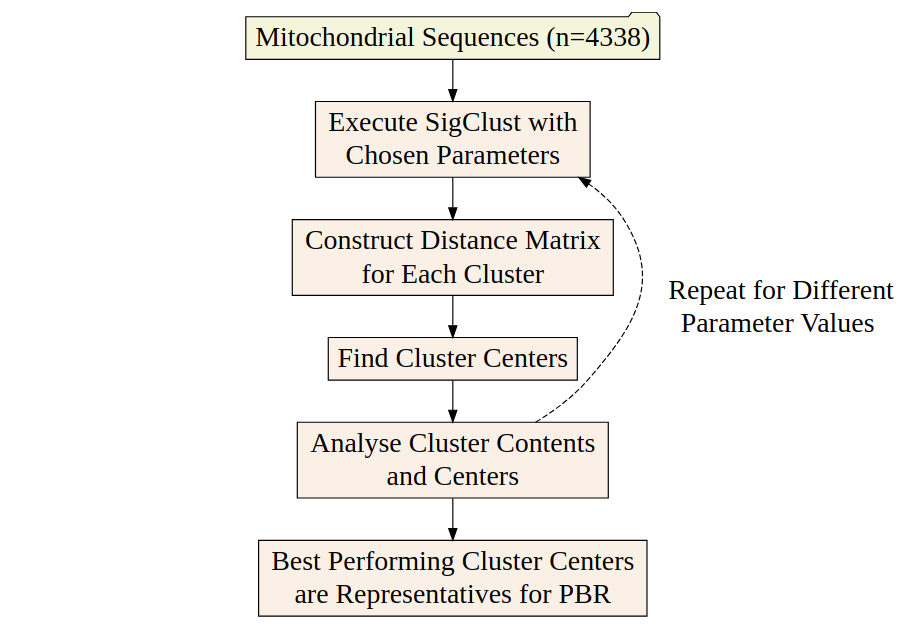
\includegraphics[width=0.9\textwidth]{flowchart.png}
    \captionsetup{margin=0.75cm}
      \caption{\textbf{\small Flow diagram demonstrating the adapted SigClust method before phylogenetic reconstruction}}
  \end{figure}

  \subsection{Phylogenetic Analysis}
  
  Upon the completion of the clustering methods mentioned, the representatives for backbone reconstruction can be used to build the phylogeny. Phylogenetic trees were constructed using IQ-TREE (multicore version 2.0.7) \cite{iqtree}, a software that utilises maximum-likelihood based phylogenetic inference. The -m MF+MERGE parameter was utilised for finding the optimal substitution model for each gene partition, and combining partitions that share the same model for efficient tree building. The molecular data was partioned by gene using the partitioner.py script from the TjCreedy phylostuff suite \cite{Tjcreedy}. The representatives for the backbone tree were aligned with 120 sequences with a well established topology which was used as a tree constraint when executing IQ-TREE. Secondly, upon the construction of a backbone tree, taxonomically homogenous and monophyletic clusters can be grafted onto their respective tip on the backbone. These subtrees are reconstructed again using IQ-TREE with identical parameters, but without any constraint.

  \section{Results}

  \subsection{Simple Kmeans Approach}

  Executing the simple kmeans approach on the entire distance matrix, for a differing number of clusters, output a varying non-zero number of sequences in each cluster. The distributions for the 50 cluster centers are only marginally shifted towards larger K2P scores, illustrating that the kmeans clustering poorly identified representatives that were most dissimilar to each other. This is even more apparent for the 100 cluster centers. F-test results show that the variances between the cluster centers and total data set distributions are significantly different ($p < 2.2 \times 10^{-16}$) for both 50 and 100 clusters, thus justifying the use of a Welch's t-test for unequal variance. Whilst these t-tests suggested significant differences between the means ($p < 2.2 \times 10^{-16}$) of the distributions for both cluster sets, a further Cohen's d test indicated small and negligible practical differences ($d = -0.318$, $d = -0.155$) between 50 and 100 clusters respectively and the distance matrix. This method showed a poor ability at finding representatives that had pairwise K2P scores at the larger end of the entire distance matrix. Therefore, it should not be developed further.

  \subsection{Adapted SigClust Algorithm}

  The SigClust algorithm executed on the COX1 gene output the members of each cluster. Subsetted distance matrices for each cluster were used to find the cluster centers to facilitate comparison in K2P score distributions. Figure 2 shows the distribution of K2P scores between the total data set and the cluster centers; in addition, density curves of differing colours show the effect of changing the kmer value.

  \begin{figure}[H]
    \centering
    \begin{subfigure}{0.5\textwidth}
        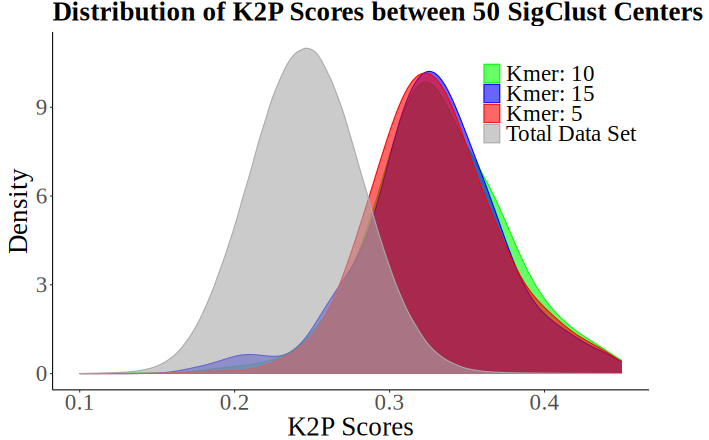
\includegraphics[width=\linewidth]{sigClust_50.png}
        \caption{50 Cluster Centers}
    \end{subfigure}%
    \hspace{-0.2cm} 
    \begin{subfigure}{0.5\textwidth}
      \raisebox{1mm}{ % Adjust the vertical position (increase or decrease the value)
      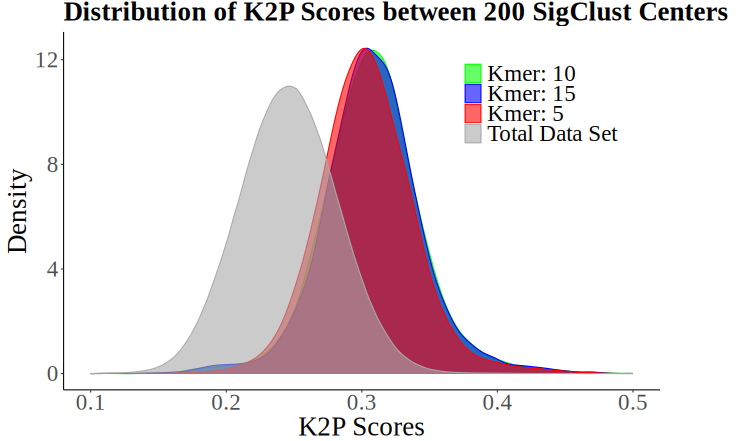
\includegraphics[width=\linewidth]{sigClust_200.png}
    }
        \caption{200 Cluster Centers}
    \end{subfigure}
    \captionsetup{margin=0.75cm}
      \caption{\textbf{\small Density plots showing the distribution of pairwise K2P scores for 50 (a) and 200 (b) SigClust cluster centers, relative to the entire distance matrix.}}
  \end{figure}

  The distribution of the 50 cluster centers are clearly significantly shifted to greater K2P scores for each kmer value. Secondly, the adapted SigClust approach also evidently found cluster centers that were dissimilar from each other for 200 clusters, likely capturing much diversity from the total sample. Increasing the number of clusters intuitively reduces the likelihood of the average pairwise similarity score deviating far from the mean of the entire distance matrix. This is backed up by additional Cohen's d scores. For all kmer values used for both sets of cluster numbers the Cohen's d scores suggest a large practical difference. Furthermore, using kmer value 5 for example, the 50 clusters gave a larger effect size than the 200 ($d = -1.580$, $d = -2.314$ respectively). Ultimately, figure 2 shows that the adapted SigClust approach shows vast improvement than the simple kmeans approach, and will be further developed henceforth. However, the density plots in Figure 3 clearly have not addressed the question on the best performing kmer value.

  Therefore, a line graph showing the mean number of taxa in each cluster against different kmer values addresses the ambiguity of the best performing kmer. Figure 3 shows a line graph for the mean number of superfamilies inside each outputted cluster. 

  \begin{figure}[H]
    \centering
    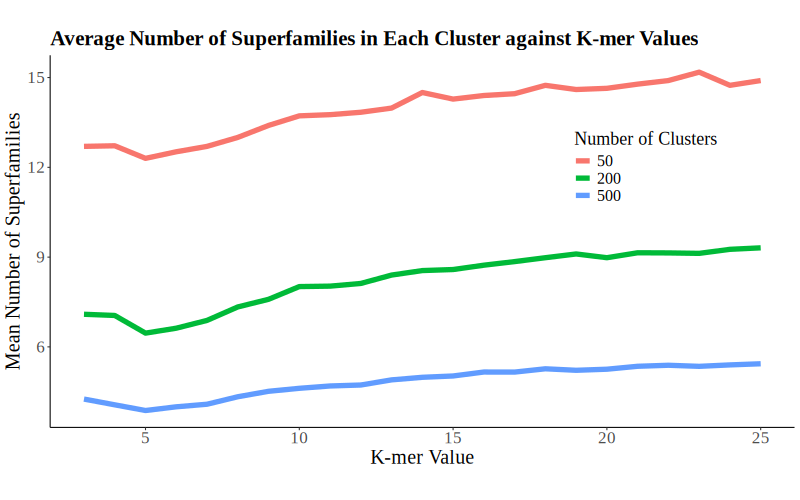
\includegraphics[width=0.9\textwidth]{Av_Super.png}
    \captionsetup{margin=0.75cm}
      \caption{\textbf{\small Line graph showing the mean number of superfamilies present in each cluster for a differing number of clusters.}}
\end{figure}

  Consistent for each different number of clusters chosen (represented by different coloured lines), kmer value 5 was best performing. At this value the mean number of different superfamilies represented in each cluster was lowest. This suggests a kmer value of 5 is best at identifying clusters that are most taxanomically homogenous at a superfamily level - indicating their potential for building monophyletic subtrees, post backbone reconstruction.

  As the desirable kmer value has been established (5), the contents of the clusters themselves, computed using this parameter value can be scrutinized. Figure 4 shows case studies for the contents of different clusters with the SigClust parameters set to kmer value 5 with 200 clusters.

  \begin{figure}[H]
    \centering
    \begin{subfigure}{0.495\textwidth}
      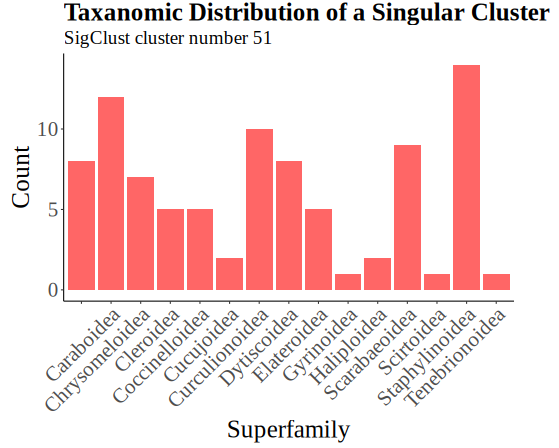
\includegraphics[width=\linewidth]{cluster_51.png}
      \caption{Case study showing a cluster with diverse contents}
    \end{subfigure}
    \begin{subfigure}{0.495\textwidth}
      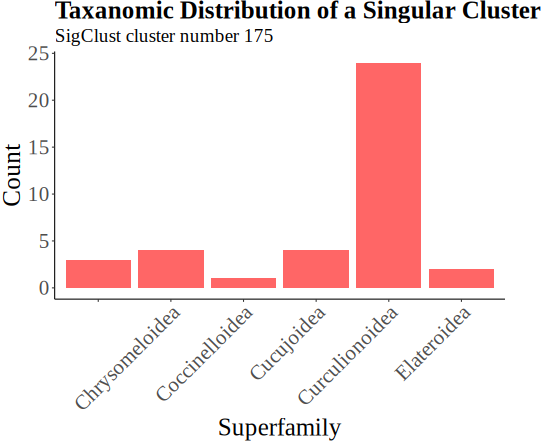
\includegraphics[width=\linewidth]{cluster_175.png}
      \caption{Case study showing a cluster with a clearly dominant taxa present}
    \end{subfigure}
    \captionsetup{margin=0.75cm}
      \caption{\textbf{\small Bar graphs showing the different taxonomic distributions of case study SigClust clusters.}}
  \end{figure}

  Figure 4 illustrates case studies for the typical contents of a SigClust cluster. Figure 4(a) shows a large cluster consisting of a broad sample of the overall biodiversity, illustrating a poor SigClust performance. Whereas, Figure 6(b) shows a better performing cluster consisting of a clearly dominant taxonomy (superfamily Curculionoidea). In addition, 41 out of the 200 clusters (20.5\%) performed perfectly to a Superfamily level consisting of sequences belonging to only one superfamily. 

  Next, the cluster centers' taxonomic distribution can be observed and is shown in figure 5. 

  \begin{figure}[H]
    \centering
    \begin{subfigure}{0.49\textwidth}
      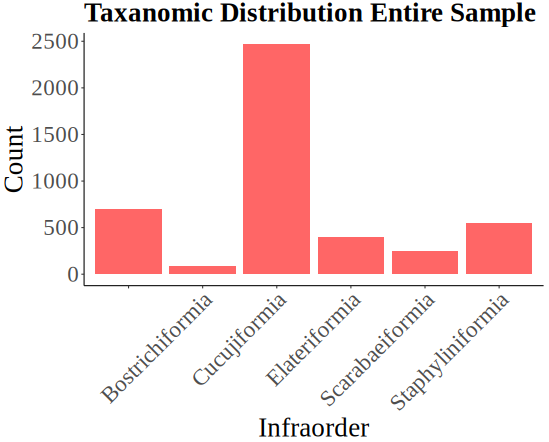
\includegraphics[width=\linewidth]{Site100_total.png}
      \caption{}
    \end{subfigure}
    \hspace{-0.3cm} 
    \begin{subfigure}{0.51\textwidth}
      \raisebox{0.5mm}{ % Adjust the vertical position (increase or decrease the value)
      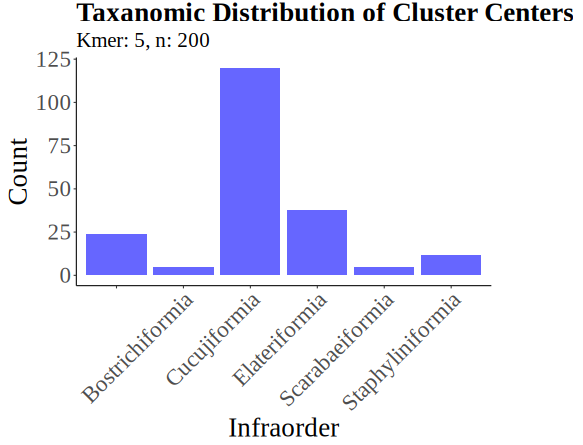
\includegraphics[width=\linewidth]{Site100_centers.png}
    }
        \caption{}
    \end{subfigure}
    \captionsetup{margin=0.75cm}
      \caption{\textbf{\small Bar graphs showing the taxonomic distributions for the cluster centers (a) and the original sample (b)}}
  \end{figure}

  Figure 5 illustrates that the cluster centers strongly replicate the taxonomic distribution of the sample - suggesting a roughly uniform and desired selection. These cluster centers, alongside sequences of the constrained topology were used to build the backbone phylogenetic tree. 

  \subsection{Phylogenetic Reconstruction}

  \begin{figure}[H]
      \centering
      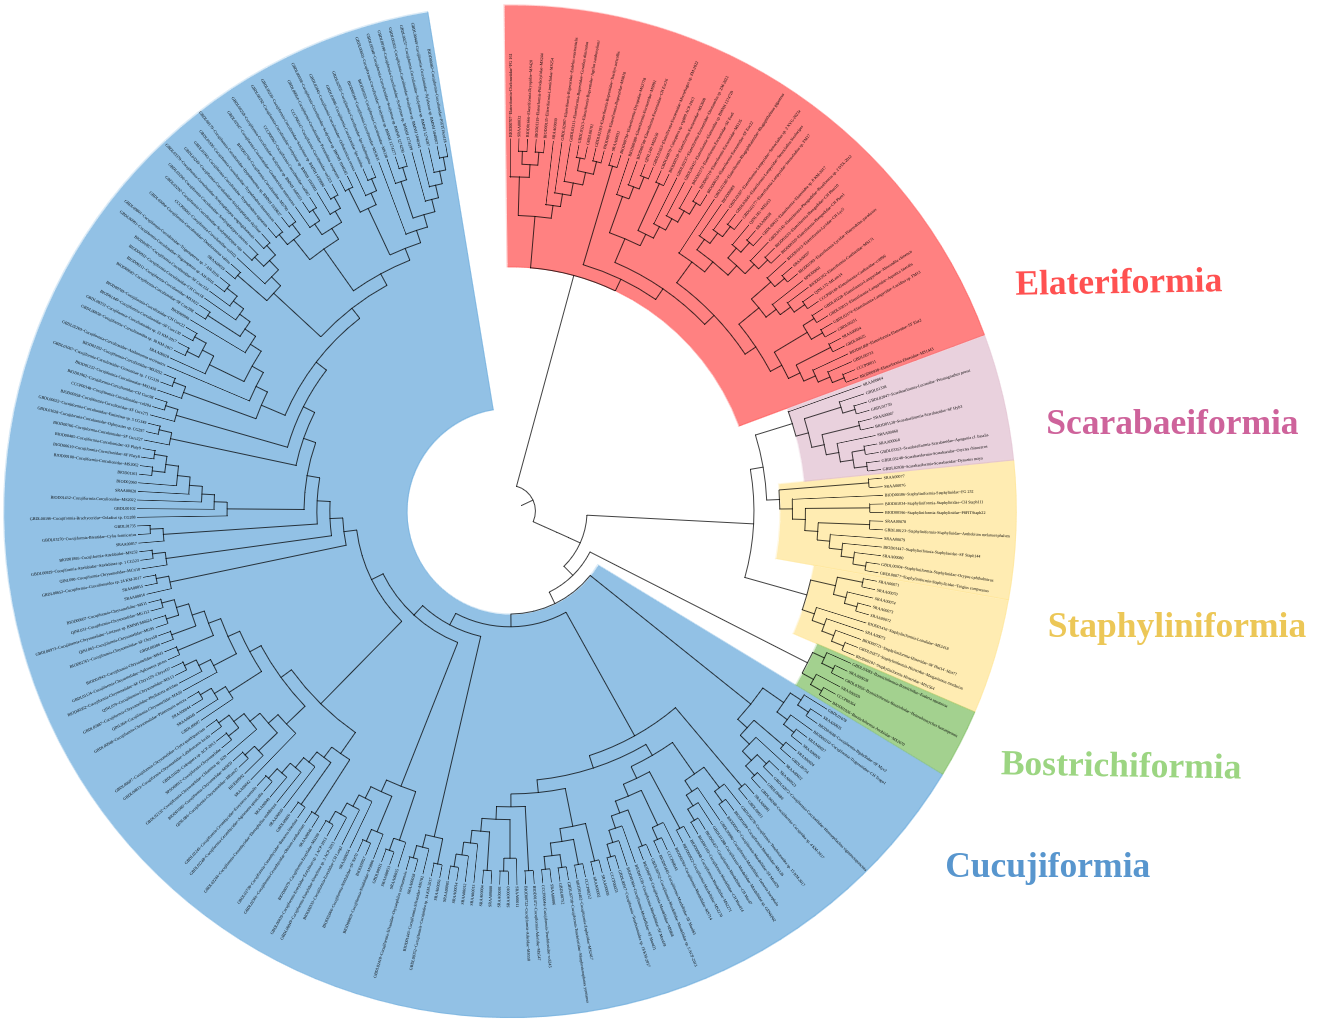
\includegraphics[width=0.95\textwidth]{bbb.png}
      \captionsetup{margin=0.75cm}
      \caption{\textbf{\small Phylogenetic cladogram illustrating the relatedness between Coleopteran infraorders.}}
  \end{figure}

  Figure 6 is a formatted phylogenetic backbone tree illustrating the diverse Coleopteran phylogeny highlighting the present infraorders. The taxonomic distribution of the original 4438 sequences is further showed in this tree. The 200 taxonomically labelled tips make up the cluster center representatives, whilst 120 non-labelled tips in figure 6 are those of the constraint tree used to increase the accuracy of the topology found in this study. The original tree file including the family and genus of all species tips in this figure are available and accessible in the code availability statement concluding this study. Once the backbone was constructed a strong performing taxonomically homogenous cluster is chosen as a case study for demonstrating how the method in this study can be performed.

  \begin{figure}[H]
    \centering
    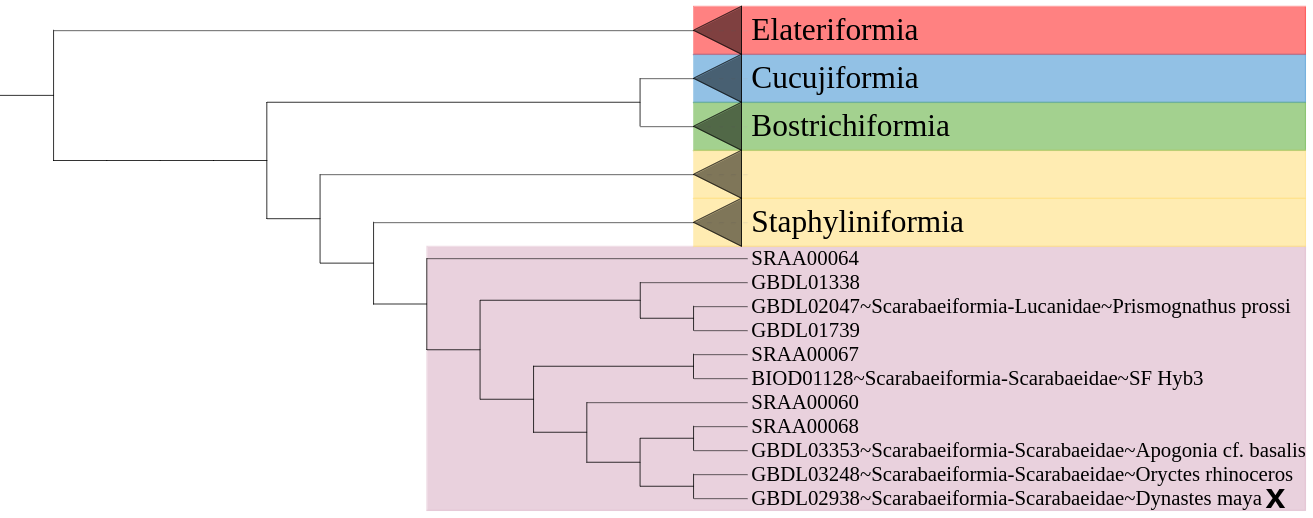
\includegraphics[width=0.95\textwidth]{bbzoomfour.png}
    \captionsetup{margin=0.75cm}
      \caption{\textbf{\small A partially collapsed tree highlighting a particular cluster center (Dynastes maya), marked with the X.}}
  \end{figure}

  Figure 7 shows an identical tree to figure 6 with condensed infraorders to highlight the chosen cluster center - marked with an X. \textit{Dynastes} maya happened to be the cluster center for an identified taxonomically homogenous cluster. A separate phylogenetic subtree is consequently built with the sequences in this cluster for refining and adding detail to the backbone.   

  \begin{figure}[H]
    \centering
    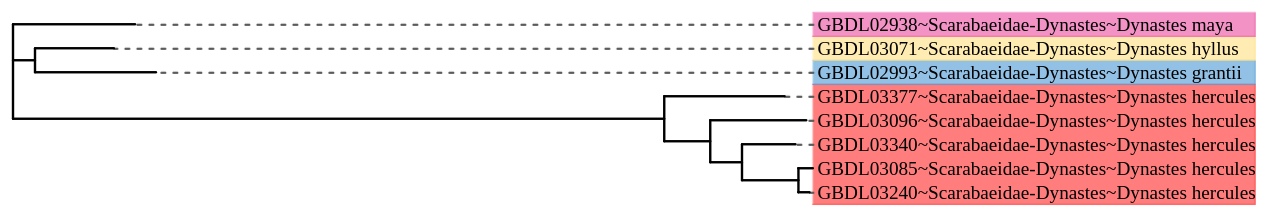
\includegraphics[width=1\textwidth]{moeny.png}
    \captionsetup{margin=0.75cm}
      \caption{\textbf{\small Phylogram showing the evolutionary relationship between species of the \textit{Dynastes} genus.}}
  \end{figure}

  Figure 8 shows an example homogenous and monophyletic subtree that adds detail to its respective cluster on the backbone. It also highlights the shortcomings of the process used to identify cluster centers. This is because \textit{Dynastes} maya is clearly not the most similar to the majority of sequences in this cluster. This is illustrated in Figure 8, as \textit{Dynastes} maya is the most distantly related sequences to all other in its cluster, despite it being found to be the cluster center.

  \section{Discussion}

  The results in this study illustrate the strengths and weaknesses of kmeans clustering in phylogenetic analyses. In addition, poor performing elements in this study may point to limitations that can be addressed in future studies. Firstly, whilst the cluster centers from the simple kmeans approach showed a pairwise K2P distribution significantly different to the total distance matrix; it is clear by the Cohen's d scores, and in comparison to consequent SigClust methods that they did not adequately capture the broad diversity of the dataset. Furthermore, the decrease in performance upon the increase in the number of clusters showed attempting this approach with more clusters would not be appropriate. This is because increasing the number of clusters creates more similarity between cluster centers as smaller clusters represent more localized portions of the data - leading to an overall increase in similarity between clusters. Faults in this simple kmeans technique must lie within either the distance matrix or the execution of kmeans clustering itself. The results from the simple kmeans approach further validate kmeans' struggle with distance matrices. It also hints at other clustering methods to be attempted on the K2P pairwise matrix. For example, another clustering method, partitioning around medoids (PAM) is a similar technique to kmeans, proven to work well with gene expression data, and is better designed for distance matrices \cite{Huang2006}.

  The pairwise distributions of the cluster centers from the adapted SigClust method convincingly outperformed, thus making redundant, the simple kmeans approach. It is clear from figure 2 that the SigClust cluster centers for all kmer values captured similar sequence similarity scores at the high extreme of the total distance matrix distribution. Thus suggesting that the cluster centers may represent sequences that are most dissimilar from each other and therefore capture the broad diversity of the data set. Another positive from the adapted SigClust method is that whilst it still requires a distance matrix, computational demands are still reduced in comparison to other clustering methods, as only subsetted matrices are required (for cluster center calculation) rather than a larger distance matrix consisting of all pairwise similarity scores in the sample.
  
  Whilst it is clear that dissimilar sequences have been selected as desired, more nuanced analysis including the taxonomy of the outputted sequences gives a greater understanding on how the clustering is performing with different parameter values. Clusters composed of sequences with minimal differences in their taxonomy are preferred. Therefore, Figure 4 illustrates how the number of different taxa (superfamilies) in each cluster changes as the kmer value increases. Its shows the effective `error' of the clustering against different kmer values. The graph therefore shows that kmer value 5 should be the set parameter for any following analysis for all numbers of clusters. Although Chappell et al. (2017) noted that different kmer values are suitable for different sets of sequences, this result was anticipated, as a kmer value of 5 is the default parameter of the algorithm and performed best in their study \cite{Chappell2017}. The contents of example clusters are illustrated as varied in figure 4. Whilst a taxanomically homogenous set of clusters would have been favourable, it is the accurate identification of cluster centers that is integral to the backbone reconstruction. However, the addition of subtrees onto the backbone would be a struggle without taxanomically homogenous clusters; therefore, some clusters are far better for tip adding than others. 

  The SigClust algorithm output clusters with taxanomically curious contents, with only 20.5\% being homogenous to a superfamily level. Furthermore, although the cluster centers' taxonomic distribution is similar to the overall samples', the adapted SigClust approach struggled to identify cluster centers that were part of the dominant taxonomy in their cluster. Whilst the approach used to find cluster centers was not effective at selecting the dominant superfamily in the cluster, it's consistency ultimately lead to the cluster centers still strongly representing the overall taxanomic distribution in the original sample - shown in Figure 5 and 6. Overall then, the experiment identified representatives capturing a similar taxanomic distribution of the infraorders than the total set. This illustrates that representatives were relatively uniformly picked from the sample as intended and that kmeans has potential to be used for selecting backbone representatives in future studies.

  The SigClust algorithm did not perform as well as intended, or as well as in the original study. The digital address of the sequences used in the original study was declared, but has since been changed, thus there is no indication on the taxonomy or relatedness between sequences or groups of sequences used in the development of the SigClust method. One can theorise that the clustering has performed poorly for a couple of reasons. Firstly, the mitogenome sequences used in this study may generally be all too similar to each other. The conversion of the sequences into kmers and their conversion to a binary format may have lost too much detail for their consequent assignments into accurate clusters \cite{Chappell2017}. Another explanation may be that there is enough diversisty within Coleoptera however there is a lack of distinct groups, synonymous with the downfall in other clustering studies. When a diverse set of sequences within one order is used, the diversity among the sample exists on a gradient rather than forming distinct groups, as is often seen with arbitrary taxonomic labels. SigClust would likely have perfomed better finding clusters from a diverse sample where there is greater discreteness between taxa in the sample. Furthermore, extreme differences between molecular mutation and speciation rates amoung different lineages suggests validating the clusters taxonomically may not have been suitable to begin with.

  In addition, the method to identify cluster centers is likely flawed as one assumes the most central observation of a cluster, from its respective distance matrix, would be of the most dominant taxa in that cluster. This was often not the case highlighting the necessity for an improved method for identifying cluster centers. Cluster centers were found using the distance matrix constructed from pairwise K2P scores. It seems more sophisticated care was required when choising how to compute this distance matrix. Firstly, K2P is a strongly backed model, however, it's execution on only the first couple codon positions may have been more suitable. This is because the third position may be saturated from massive divergence that renders it useless, and often detrimental to phylogenetic analyses \cite{orlov}. Saturation is an important factor in phylogenetic analysis and is known to be particularly prevalent for the COX1 gene. Saturation is a problem as it leads to long-branch attraction due to sequences' evolutionary convergent biases \cite{Yuan2022}. Extra care could have been taken by testing for saturation \cite{YUAN201699} before deciding if it should be removed before the conduction of phylogenetic analysis in this study. This potential bias may even have been amplified by the use of only one mitochondrial PCG (COX1) in this study. The use of only a single gene for the distance matrix suggests the study could have employed software for finding the optimal model of evolution \cite{} before computing the distance matrix. Though K2P is often appropriate other models of evolution may have been more suited to the dataset. Furthermore, alternative resolutions to this issue may include executing the SigClust algorithm on the entire mitogenomes, or their concatenated PCGs. In addition, the third codon position has a tendancy to become saturated and can be addressed by only including position one and two in the distance matrix construction and the SigClust implementation.

  In hindsight, another potential limitation of the study was incorrectly prioritising the kmer value parameter over the number of clusters parameter. The cluster contents for a changing number of clusters were analysed for comparison; however, ultimately 200 clusters was an arbitrarily chosen parameter value predicted to be suitable for the original sample and backbone reconstruction task. More clusters would have resulted in a more diverse backbone, but at a computational cost. Furthermore increasing the number of clusters also increases the likelihood of overfitting. A too great number of clusters cause the algorithm to form clusters encapsulating the noise in the data, rather than the underlying patterns. An improvement in future studies would be to perform the 'knee method' for finding the optimal number of clusters. This would address the trade-off between the amount of error (mean number of different taxa) in each cluster and the overall number of clusters, helping to identify a parsimonious balance that maximizes the accuracy of the model whilst minimising the likelihood of overfitting. 

  \section{Conclusion}

  In conclusion, the results in this exploratory investigation show the potential for using kmeans clustering for identifying representatives for backbone reconstruction. The computation of cluster centers that have an associated monophyletic or taxonomically homogenous cluster, is a novel idea that should be explored further in future studies that aim to solve the challenge of large phylogenetic tree building. Whilst there were few taxonomically pure clusters, this study still showed an example subtree, whose phylogeny could be more broadly observed alongside the backbone. Furthermore, the method in this study is a flexible and efficient solution to building large trees. This is because extra detail may be added via subtrees wherever is desired, instead of building all of the subtrees - thus saving computational time. 

  \section{Data and Code Availability}

  All code written and information on the packages used for the analyis and write-up in this thesis can be found in the following GitHub repo: \\
  https://github.com/SamSmithImperial/CMEECourseWork/Project

  More information regarding the Site 100 data used in this study can be found at: www.site100.org

  \section{Acknowledgements}

  I would firstly like to thank Professor Alfried Vogler and his lab group for welcoming me into the Natural History Museum and guiding me through this MSc thesis. Thank you for the opportunity to work in this team and contribute to weekly lab meetings. Secondly, I would like to thank Professor Samraat Pawar and Professor James Rosindell for co-organising, delivering and supporting me through this MSc in Computational Methods in Ecology and Evolution.

  \bibliographystyle{plain}
  
  \bibliography{Bibliography.bib}

  \rule{\linewidth}{0.1mm}
  \begin{center}
    End of Document
  \end{center}

\end{document}